\documentclass[letterpaper,times]{IONconf}

%% Math
\usepackage{amsmath}
\usepackage{amssymb}
\usepackage{bm}

%% Graphics and tables
\usepackage{graphicx}
\usepackage[justification=centering]{caption}
\usepackage{subcaption}
\usepackage{array}
\usepackage{booktabs}
\usepackage{multirow}

%% Algorithms
\usepackage{algorithm}
\usepackage{algpseudocode}

%% Symbols (for \ding{55} cross-mark in the ablation table)
\usepackage{pifont}

%% URLs and references
\usepackage{url}
\usepackage{natbib}
\usepackage[hidelinks]{hyperref}

\graphicspath{{figures/}}
\DeclareGraphicsExtensions{.pdf,.png,.jpg,.jpeg}


\title{Perception-Aware Path Planning for Lunar Rover Autonomy: \\
Active Loop-Closure Engineering via Keyframe-Revisit Detours}

\author{
    Santiago~Thorup, \textit{Stanford~University}%
    }


\begin{document}

\maketitle


\section*{biography}

\biography{Santiago Thorup}{Santiago Thorup is a graduate student in the Department of Aeronautics and Astronautics at Stanford University, working on autonomous navigation and reachability analysis for space systems. This work was conducted as the final project for AA278: Multi-Robot Systems and Decentralized Control, Spring 2026.}


\section*{Abstract}

Autonomous lunar rovers operate without satellite navigation and must therefore localize against on-board sensing alone. Visual-inertial SLAM systems used for this purpose accumulate drift roughly proportional to distance traveled --- at the multi-kilometer scales planned for upcoming lunar surface missions, the resulting localization error can reach tens of meters unless actively bounded. Loop closure, the SLAM mechanism by which re-encountering a previously mapped region corrects accumulated drift, is the principal software-only mitigation, but it requires the rover's mission plan to physically revisit feature-rich, visually distinctive terrain. Heritage slope-aware planners optimize for traversability and energy rather than perceptibility, and rarely produce trajectories that fire loop closures incidentally. We present a perception-aware global planner that engineers loop closures through two composable mechanisms. First, the A* edge cost is augmented with DEM-derived perception terms --- a shadow-avoidance penalty and a traversability-safety penalty --- that route the rover through sunlit, feature-stable corridors while staying clear of unsafe rocky regions. Second, an online keyframe-revisit detour mechanism monitors the SLAM backend's loop-closure history and, after a configurable drift budget elapses without a loop closure, splices a detour through a previously visited keyframe back into the planned tour, then resumes. The detour target is driveable by construction (the rover already went there) and loop-closure-eligible by construction (the backend already stored a keyframe there). On a six-sub-goal perimeter tour in the Stanford NavLab Lunar Autonomy Challenge simulator, the proposed planner achieves SLAM RMSE of 0.14~m on a 139~m trajectory --- a 4.16$\times$ reduction in absolute localization error and a 5.55$\times$ reduction in per-meter drift relative to a slope-aware A* baseline, despite a 35\% longer path. Twenty of the 54 loop closures fired during the run bind late-mission keyframes back to the first 10\% of the trajectory, providing the global drift correction the heritage planner cannot.


\section{Introduction}

Autonomous lunar rovers operating on the south polar region of the Moon cannot rely on satellite navigation: GNSS does not reach the Moon, and a dedicated lunar GNSS infrastructure does not yet exist. Localization is derived instead from on-board sensing --- typically a fusion of stereo visual odometry, an inertial measurement unit, and wheel encoders --- closed into a SLAM pose graph that grows monotonically with mission duration~\citep{campos2021orbslam3, qin2018vins}. The Stanford NavLab Lunar Autonomy Challenge (LAC) framework adopted in this work follows this archetype: stereo SuperPoint~\citep{detone2018superpoint} features matched by LightGlue~\citep{lindenberger2023lightglue}, with relative-pose constraints accumulated in a GTSAM~\citep{dellaert2012gtsam} factor graph and optimized by Levenberg--Marquardt.

Visual-inertial SLAM systems are known to drift at 0.5--1\% of distance traveled in well-instrumented terrestrial conditions. On the lunar surface --- where regolith is texture-poor in shadow, the sun grazes the horizon at altitude below 2$^\circ$, and rocks are sparse but visually rich --- drift is empirically worse. NASA's Volatiles Investigating Polar Exploration Rover (VIPER)~\citep{nasa2022viper} plans a multi-kilometer south-polar traverse; even sub-1\% drift accumulates to hundreds of meters of localization error, well beyond the sub-meter tolerances required for sample collection and infrastructure emplacement.

The standard mitigation is \emph{loop closure}: when the rover re-observes a previously mapped region, the SLAM backend matches the current imagery against an earlier keyframe and adds a relative-pose constraint that pulls accumulated drift back toward the original anchor. Loop closures are the only mechanism in our pipeline that \emph{bounds} SLAM error globally rather than letting it grow monotonically with distance. They are not free: the rover must physically revisit terrain that is (a) visually distinctive enough to produce successful feature matches, and (b) geometrically close enough to a stored keyframe for the backend's proximity-based candidate search to find it. A rover whose mission plan never revisits its own trail will fire few or no loop closures, and its localization will drift unbounded.

This work asks: \emph{can the global path planner be made loop-closure aware?} The dominant lunar planner archetype --- slope-aware A* over a digital elevation model (DEM)~\citep{stanford_aa278_hw3} --- optimizes for traversability and energy. It cannot predict whether a planned leg will leave the rover visually blind, and it produces trajectories that fire loop closures only incidentally. We propose to instead treat the global planner itself as a \emph{loop-closure engineering tool}: route the rover through cells the DEM predicts to be sunlit and visually stable, and, when SLAM has been drifting for too long without a loop closure, actively detour through a past keyframe to engineer one.

Our contributions are threefold:
\begin{enumerate}
    \item A perception-aware A* edge cost that composes a slope penalty (the heritage baseline), a DEM-derived shadow-avoidance term, and a traversability-safety term. We show that the shadow term --- the simplest of three perception-cost candidates we evaluate --- is the most robust.
    \item An online \emph{keyframe-revisit} detour mechanism that, when triggered by elapsed-steps-since-last-loop-closure, splices a detour through a previously visited keyframe into the planned tour. We contrast this against a \emph{tight-anchor} alternative that targets DEM-predicted feature-rich cells, and show that the keyframe-revisit tactic substantially outperforms it.
    \item A 3$\times$3 ablation matrix on the LAC simulator, demonstrating that the composite \emph{Shadow~$+$~Safety global cost~$+$~Keyframe-Revisit detour} configuration achieves 0.14~m SLAM RMSE on a 139~m tour --- a 5.55$\times$ per-meter drift reduction over the slope-aware A* baseline.
\end{enumerate}

A central mechanistic finding sharpens the contribution: 20 of the 54 loop closures fired by the winning variant bind late-mission keyframes back to the first 10\% of the trajectory, near the GTSAM prior pose. These cross-trajectory bindings --- not mid-trajectory loop closures --- are what enables \emph{global} drift correction, and they appear because the keyframe-revisit detour drives the rover near old keyframes that the SLAM-estimated pose can still find geometrically.

The remainder of the paper is organized as follows. Section~\ref{sec:related} surveys related work in visual-inertial SLAM, active perception, and lunar planning. Section~\ref{sec:problem} states the planning and SLAM problem formally. Section~\ref{sec:approach} describes the perception-aware cost function and the keyframe-revisit detour mechanism. Section~\ref{sec:results} presents the headline results, mechanism analysis, and the full ablation matrix. Section~\ref{sec:conclusion} concludes; Section~\ref{sec:future} outlines extensions. All code, configurations, and figures are available at the project repository~\citep{thorup2026repo}.


\section{Related Work}
\label{sec:related}

\textbf{Visual-inertial SLAM and loop closure.} Modern visual-inertial SLAM systems --- ORB-SLAM3~\citep{campos2021orbslam3}, VINS-Fusion~\citep{qin2018vins}, OpenVINS~\citep{geneva2020openvins}, Kimera~\citep{rosinol2020kimera} --- share a common architecture: a tightly coupled visual-inertial frontend feeds a pose-graph backend optimized by iSAM2 or GTSAM~\citep{dellaert2012gtsam}. The LAC reference SLAM follows this archetype. Loop-closure detection in the LAC backend is \emph{geometric}: a candidate must lie within \texttt{LC\_DIST\_THRESHOLD}~$=$~1~m and \texttt{LC\_ANGLE\_THRESHOLD}~$=$~5$^\circ$ of the current SLAM-estimated pose. Appearance-based loop-closure search using bag-of-words descriptors (DBoW2/DBoW3~\citep{galvez2012dbow2}) or learned global descriptors (NetVLAD~\citep{arandjelovic2016netvlad}) is the prevailing alternative, robust to large SLAM drift, but requires an additional descriptor pipeline that we did not modify. The implication for our work is structural: the LAC backend's geometric trigger \emph{cannot detect} a true revisit once accumulated drift exceeds 1~m. Our planner-side mechanism is designed to operate within this constraint rather than fix it.

\textbf{Active and perception-aware SLAM.} \citet{carrillo2012} formalize active SLAM as a problem of choosing control actions to maximize information gain about the map and pose, with D-optimality (maximizing $\det \Lambda$) as the canonical objective. Subsequent work generalizes to coverage-aware exploration~\citep{stachniss2009robotic}, next-best-view planning for 3D reconstruction~\citep{bircher2016receding}, and belief-space planning~\citep{platt2010belief, indelman2015planning}. The closest priors to our approach are perception-aware planners that augment traversability cost with a feature-richness reward computed from imagery or a learned predictor~\citep{mostegel2014active, costante2018perception, zhang2018perception}. These typically operate either \emph{locally} (next-best-view) or over a \emph{pre-mapped} environment. We differ in that our feature-density prediction is computed \emph{a priori} from a DEM, with no prior visual observation of the terrain. This is appropriate for lunar planning because the DEM is the only a-priori knowledge available; orbital imagery from the Lunar Reconnaissance Orbiter Narrow Angle Camera~\citep{robinson2010lro} provides comparable terrain knowledge for actual lunar missions.

\textbf{Lunar rover localization and planning.} The lunar rover navigation literature acknowledges drift as the dominant localization risk~\citep{petersen2022lunar, jpl_viper_planning}, with mitigations historically focused on periodic operator-supervised stop-and-localize against orbital imagery, IMU-aided VO, or operator-in-the-loop waypoint adjustment. To our knowledge, none treats the global planner itself as a loop-closure engineering tool. The slope-aware A* used as our baseline, derived from the Stanford AA278 Homework~3 Problem~4 formulation~\citep{stanford_aa278_hw3}, is representative of operational lunar planners. Our two principal contributions are (i)~demonstrating that \emph{shadow avoidance} is a simpler and more robust DEM-derived perception cost than the natural alternative of routing toward predicted-feature-rich cells, and (ii)~showing that an \emph{online keyframe-revisit detour} suffices to actively engineer loop closures in a tour-style mission.


\section{Problem Statement}
\label{sec:problem}

\subsection{Environment and Assumptions}
A rover navigates a 2D ground plane $(x, y) \in [-L, L]^2$ with $L = 13.5$~m (the LAC operational area), discretized at cell width $\Delta = 0.15$~m for a 180$\times$180 grid. The rover has access to a ground-truth digital elevation model $Z : \mathbb{R}^2 \to \mathbb{R}$ on the same grid, plus a known sun azimuth $\phi_s$ and altitude $\alpha_s$. LAC fixes $\phi_s = 263.575^\circ$ CCW from $+x$ and $\alpha_s = 1.488^\circ$ for every preset; only the elevation map changes between presets. The rover's pose is estimated by an on-board SLAM system whose state is a sequence of keyframe poses $\{X_i\}_{i=1}^K$ in a factor graph $\mathcal{G} = (\mathcal{V}, \mathcal{E})$ with VO odometry factors and loop-closure factors. The SLAM estimate $\hat{X}_i$ may differ from the true pose $X_i^*$ by an accumulated drift $\|\hat{X}_i - X_i^*\|_2$.

The mission is a \emph{tour}: an ordered sequence of $M$ sub-goals $\mathcal{G}_{\text{tour}} = (g_1, \dots, g_M)$ with $g_k \in \mathbb{R}^2$. The rover must visit each sub-goal in order, starting from a spawn pose $x_s$. The closed-loop tour case sets $g_1 = g_M$ so the rover returns to the start.

\subsection{Global Planning}
The global planner produces a waypoint sequence $W = (w_0, \dots, w_N)$ with $w_0 = x_s$ and $w_N = g_M$, generated by an A* graph search between each consecutive sub-goal and concatenated to 2~m spacing. The local controller (LAC's unmodified ArcPlanner) handles safe steering between waypoints and is treated as a black box. The A* edge cost between adjacent cells $n_1, n_2$ is

\begin{equation}
\label{eq:edge_cost}
\begin{aligned}
c(n_1, n_2) = d \cdot \Big(
    & 1
    + \alpha \, \big(\theta(n_2)/\theta_{\text{ref}}\big)^2 \\
    & + \beta \, \big(1 - \rho(n_2)\big) \\
    & + w \, \mathrm{trav}(n_2)
    + s \, \mathrm{shadow}(n_2)
\Big),
\end{aligned}
\end{equation}

where $d = \|n_2 - n_1\|_2$, $\theta(n_2)$ is the local slope at $n_2$ from DEM gradients, $\theta_{\text{ref}} = 10^\circ$, and a hard infeasibility filter rejects neighbors with $\theta > \theta_{\max} = 20^\circ$. The slope weight $\alpha = 2$ matches the heritage baseline. The remaining terms are the perception contributions: $\rho(n)$ is a \emph{look-ahead} feature-density predictor averaged over forward distances along the entry direction (Sec.~\ref{sec:approach}), $\mathrm{trav}(n) \in [0, 1]$ is the normalized roughness at $n$, and $\mathrm{shadow}(n) \in \{0, 1\}$ indicates whether $n$ receives direct sunlight under the fixed sun direction. The weights $(\beta, w, s)$ are configurable and select between the three cost variants studied (Sec.~\ref{sec:variants}). The multiplier $(1 + \cdots)$ is always $\ge 1$, so the Euclidean distance heuristic remains admissible.

\subsection{SLAM, Loop Closure, and the Localization Metric}
On each new keyframe, the LAC backend adds a VO odometry factor to the previous keyframe and searches for loop-closure candidates among earlier keyframes (excluding the most recent $\texttt{LOOP\_CLOSURE\_EXCLUDE} = 10$) whose SLAM-estimated position is within \texttt{LC\_DIST\_THRESHOLD}~$=$~1~m and whose orientation differs by less than 5$^\circ$. For each candidate, LightGlue is run against the candidate's stored features; if at least 100 matches at score $\ge 0.5$ survive, a $\texttt{BetweenFactorPose3}$ is added with diagonal noise sigmas $[8.7 \times 10^{-4}~\text{rad}, 5 \times 10^{-3}~\text{m}]$ on rotation and translation. The pose graph is then re-optimized by Levenberg--Marquardt. Note that the LC search uses the \emph{SLAM-estimated} pose, not ground truth: once accumulated drift exceeds 1~m, the trigger cannot detect a true revisit. This structural limit bounds the operational envelope of any planner-side mechanism that relies on it firing.

The end-of-mission localization error is the RMSE between SLAM and ground-truth trajectories,

\begin{equation}
\label{eq:rmse}
\mathrm{RMSE} = \sqrt{\frac{1}{N} \sum_{i=1}^N \|\hat{X}_i - X_i^*\|_2^2}.
\end{equation}

We also report per-meter drift $\mathrm{RMSE}/L_{\text{path}}$, which normalizes for variants whose ground-truth trajectory lengths differ by tens of meters; absolute RMSE on a 50~m path is not comparable to RMSE on a 140~m path.


\section{Approach}
\label{sec:approach}

\subsection{DEM-Derived Perception Predictor}
\label{sec:predictor}

From the DEM we compute a per-cell roughness field $r(n)$ (local elevation standard deviation in a 5-cell window) and a binary shadow mask $\mathrm{shadow}(n) \in \{0, 1\}$ obtained by ray-casting from each cell toward the sun direction at altitude $\alpha_s$ and checking for occlusion. The base predictor is

\begin{equation}
\rho_{\text{full}}(n) = r(n) \cdot \big(1 - \mathrm{shadow}(n)\big),
\end{equation}

normalized per-map by the 95th percentile of finite values to give $\rho_{\text{norm}}(n) \in [0, 1]$. The look-ahead predictor at cell $n_2$ entering from $n_1$ averages $\rho_{\text{norm}}$ at three forward distances along the entry direction $\hat{u} = (n_2 - n_1)/\|n_2 - n_1\|$:

\begin{equation}
\rho(n_2) = \frac{1}{|\mathcal{D}|} \sum_{d \in \mathcal{D}} \rho_{\text{norm}}\!\big(n_2 + d\hat{u}\big), \;\; \mathcal{D} = \{1.5, 2.5, 3.5\}~\text{m}.
\end{equation}

\textbf{Phase~0 validation.} Before evaluating the planner end-to-end, we validated whether $\rho$ correlates with observed feature count. A safe collector agent traversed a serpentine raster on LAC preset~7, capturing 10{,}565 stereo frames. For each frame we computed the SuperPoint feature count and four candidate predictor values (pose-$\rho$ and look-ahead $\rho$ at $d \in \{1.5, 2.5, 3.5, 4.0\}$~m). The strongest correlate was look-ahead $\rho$ at $d = 1.5$~m, with $|\text{Pearson}| = 0.29$. Mean feature count rose monotonically with the roughness quartile of the look-ahead cell (Q1:~658 features; Q4:~757 features). Critically, pose-$\rho$ \emph{anti-correlated} with features while look-ahead $\rho$ correlated positively --- a finding that drove the choice to reward look-ahead $\rho$ at the cell the camera is \emph{looking at}, not the cell the rover is \emph{on}. A Pearson coefficient near 0.25 is borderline-positive: the predictor captures real structure but is not strong enough to drive a global cost on its own. This observation motivated both the traversability-safety penalty and the shadow-only variant introduced below.

\textbf{Map illustration.} Figure~\ref{fig:perception_field} shows the predictor inputs on LAC preset~6 (the evaluation preset). The left panel is normalized roughness (the feature-density predictor with no shadow applied); the right panel is the binary shadow mask. The strongly anisotropic shadow pattern follows from the fixed solar geometry: a sub-2$^\circ$ sun altitude produces long shadows from every elevation feature.

\begin{figure}[t]
\centering
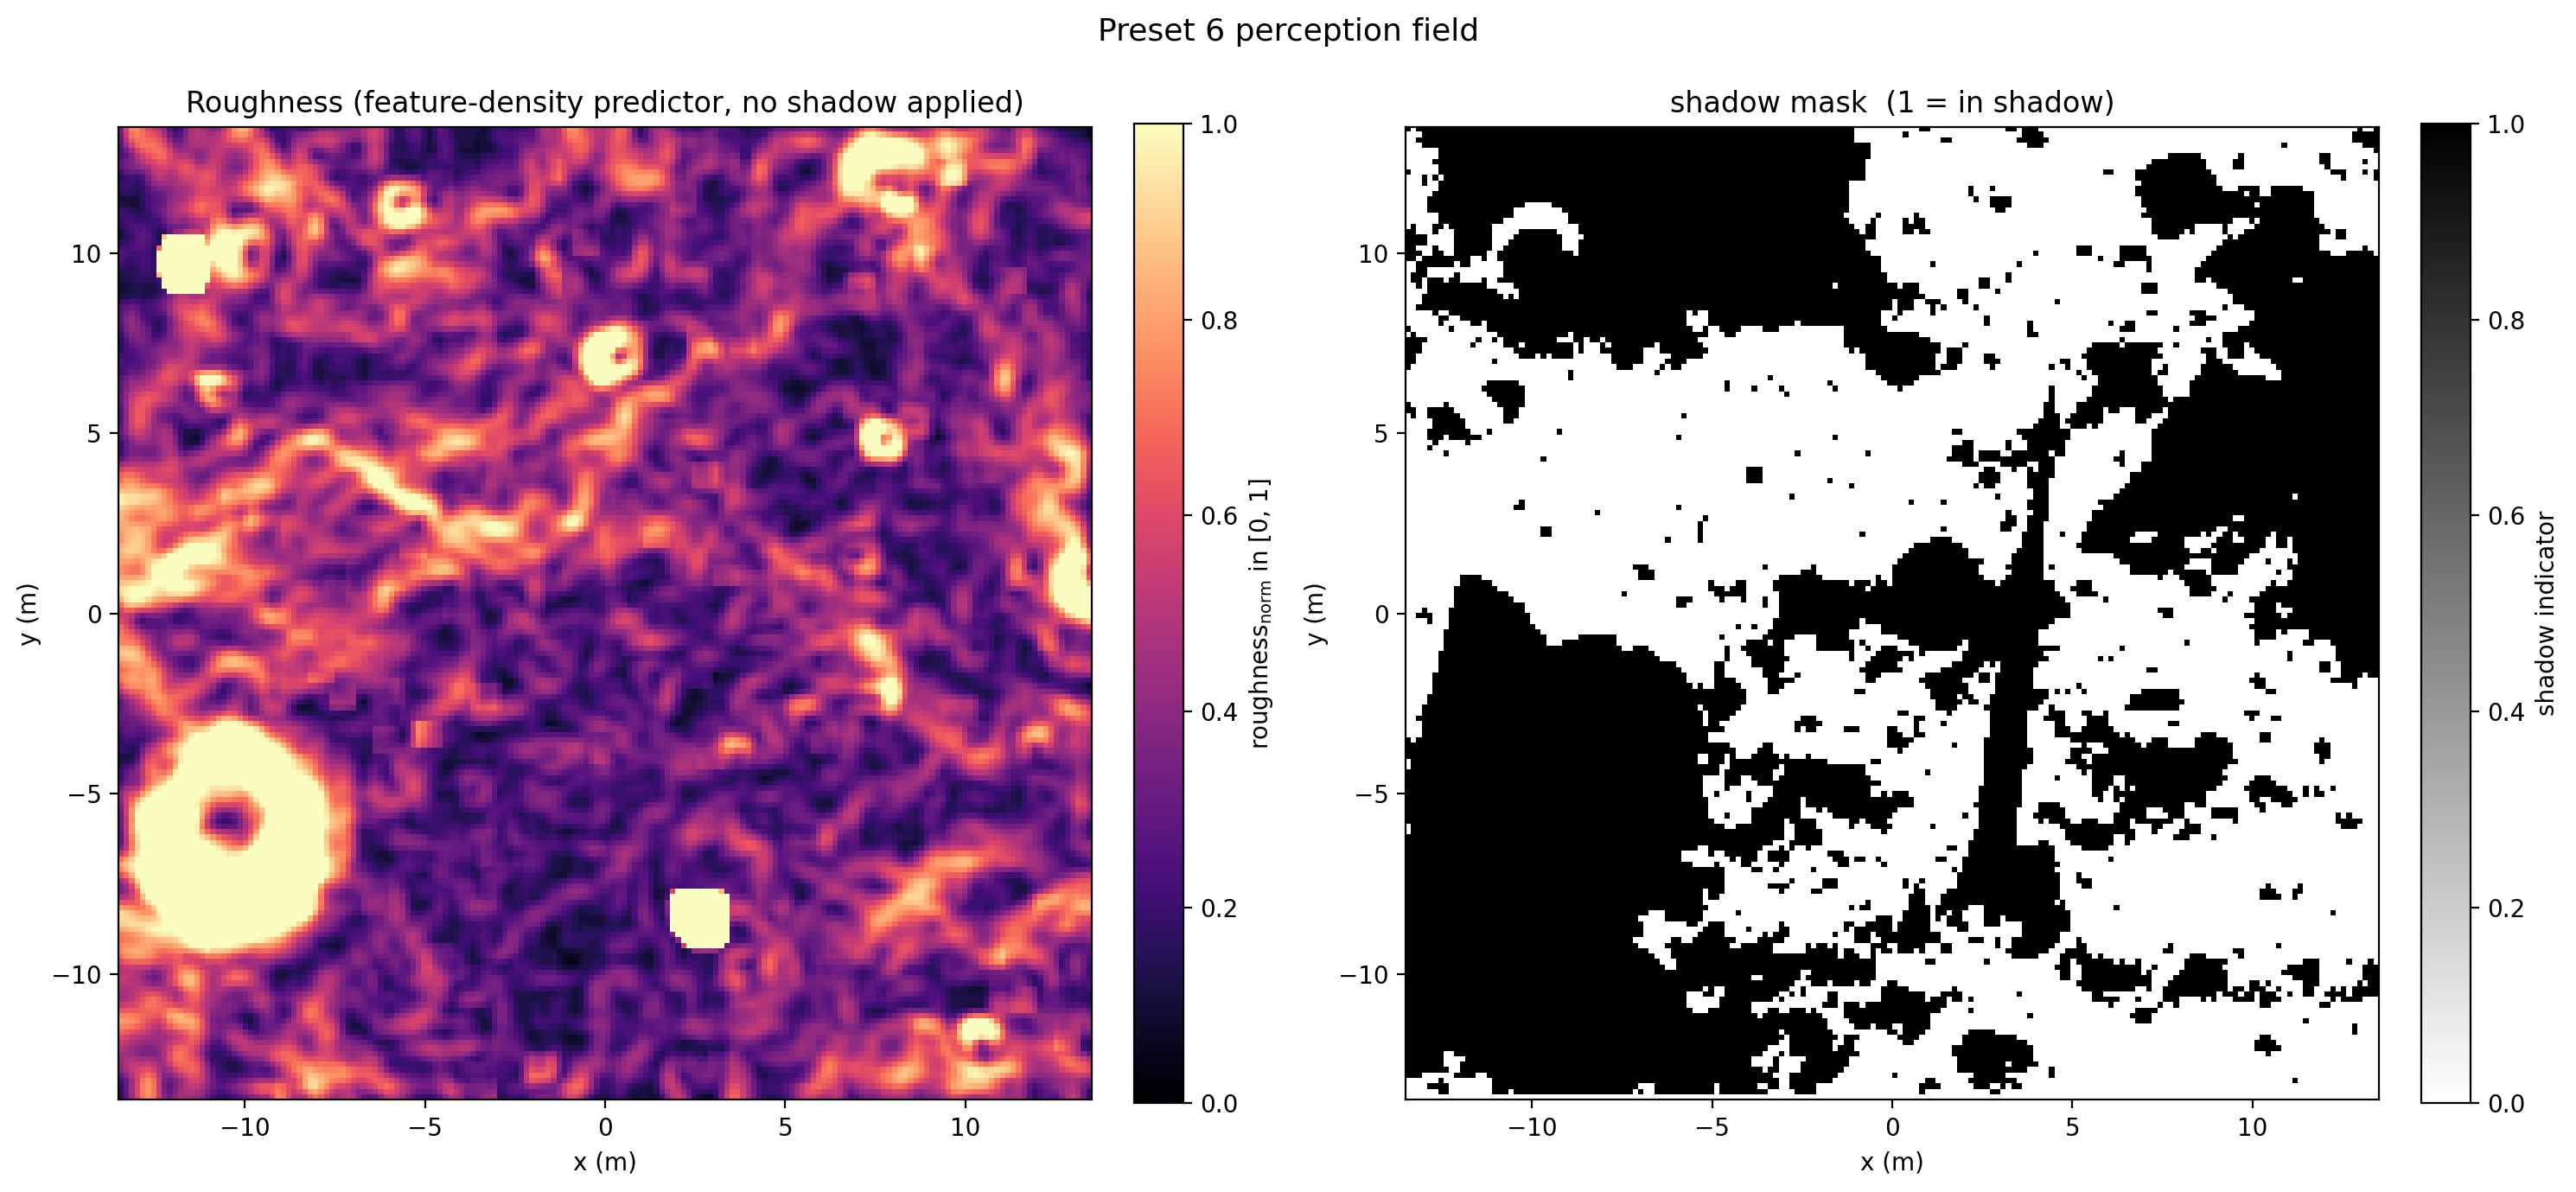
\includegraphics[width=\linewidth]{04_perception_field_preset6}
\caption{DEM-derived perception inputs on LAC preset~6. \textbf{Left:} normalized roughness field $\mathrm{trav}(n)$, the basis of the feature-density predictor (shown without the shadow term applied so the underlying structure is visible). \textbf{Right:} binary shadow mask under the fixed solar geometry ($\phi_s = 263.575^\circ$, $\alpha_s = 1.488^\circ$). The grazing sun produces long, anisotropic shadows from every elevation feature.}
\label{fig:perception_field}
\end{figure}

\subsection{Three Global-Cost Configurations}
\label{sec:variants}

Equation~\eqref{eq:edge_cost} parameterizes a family of A* costs by the triple $(\beta, w, s)$ with $\alpha = 2$ and $\theta_{\text{ref}} = 10^\circ$ held constant. We evaluate three concrete settings (Table~\ref{tab:variants}):

\begin{itemize}
    \item \textbf{Baseline} ($\beta = 0$, $w = 0$, $s = 0$): the heritage HW3-P4 slope-aware A* --- shortest slope-feasible path.
    \item \textbf{High Feature} ($\beta = 2$, $w = 8$, $s = 0$): route toward look-ahead-predicted feature-rich cells, with a heavy traversability penalty preventing the planner from steering into rocky cells. The penalty is necessary: high-$\rho$ cells co-occur with rocky cells (the predictor's roughness component is its source of variance), and without it the rover stalls.
    \item \textbf{Shadow Avoidance} ($\beta = 0$, $w = 0$, $s = 2$): drop $\rho$ entirely and rely only on the shadow indicator. Conceptually the simplest cost --- \emph{prefer sunlit cells}. We later add a safety term to produce the composite \emph{Shadow~$+$~Safety} variant ($\beta = 0$, $w = 4$, $s = 6$) that constitutes the headline winner.
\end{itemize}

\begin{table}[t]
\renewcommand{\arraystretch}{1.2}
\caption{Perception-cost weights for the three global-cost variants studied. All share $\alpha = 2$ and $\theta_{\text{ref}} = 10^\circ$.}
\label{tab:variants}
\centering
\begin{tabular}{lccc}
\toprule
Variant & $\beta$ (look-ahead $\rho$) & $w$ (roughness) & $s$ (shadow) \\
\midrule
Baseline (HW3-P4)        & 0 & 0 & 0 \\
High Feature             & 2 & 8 & 0 \\
Shadow Avoidance         & 0 & 0 & 2 \\
\textbf{Shadow + Safety} & 0 & 4 & 6 \\
\bottomrule
\end{tabular}
\end{table}

\subsection{Online Keyframe-Revisit Detour}
\label{sec:detour}

The second mechanism is an online detour triggered when SLAM has been drifting for too long without a loop closure. A SLAM-state provider closure is injected into the planner from the agent at construction; on each step it returns the current pose-graph index $i$, the list of loop closures fired so far $\{(a_k, c_k)\}$, and the LC-eligible keyframe positions $\mathcal{K}_{\text{eligible}} = \{X_j : j \le i - 10\}$ (the most recent 10 are excluded to match the backend's geometric search window).

The detour fires when

\begin{equation}
\Delta t_{\text{LC}} := i - c_{|\text{LC}|} > T_{\text{LC}}, \quad T_{\text{LC}} = 400,
\end{equation}

where $c_{|\text{LC}|}$ is the index of the most recent loop closure (or 0 if none has yet fired). The detour target is selected from $\mathcal{K}_{\text{eligible}}$ as the keyframe $X_j$ in the proximity band $[2, 8]$~m of the current SLAM pose that minimizes the additional path length

\begin{equation}
\Delta L_j = \|p \!\to\! X_j\| + \|X_j \!\to\! g_k\| - \|p \!\to\! g_k\|,
\end{equation}

where $p$ is the current SLAM pose and $g_k$ is the next un-reached sub-goal. The planner then \emph{replaces} (not patches) the remaining waypoint list with a freshly planned A* path
\[
p \to X_j \to g_k \to g_{k+1} \to \dots \to g_M,
\]
resampled to 2~m spacing. The first sample of the new path is dropped because it lies at the current pose (the rover would otherwise advance instantly); a sub-goal-index offset preserves the global tour counter across re-plans.

The detour is marked \emph{verified-success} when the SLAM backend fires a loop closure whose anchor keyframe lies within $2 \times \texttt{LC\_DIST\_THRESHOLD} = 2$~m of the detour target. Otherwise, after a per-detour cap of $T_{\max} = 1500$ steps, the target is added to a per-leg blacklist and the rover resumes the tour. To prevent unbounded detour loops on a single leg, at most three detours fire per sub-goal; the counter resets when the sub-goal advances. The per-waypoint stuck-detection timeout is widened from 2{,}000 to 4{,}000 steps during an active detour, because detour legs typically require more ArcPlanner replanning around rocks and benefit from a longer recovery budget. The full mechanism is summarized in Algorithm~\ref{alg:detour}.

\begin{algorithm}[t]
\caption{Online Keyframe-Revisit Detour}
\label{alg:detour}
\begin{algorithmic}[1]
\Require pose $p$, next sub-goal $g_k$, SLAM state $\{i,\, \{(a_l, c_l)\},\, \mathcal{K}_{\text{eligible}}\}$
\Require parameters $T_{\text{LC}}{=}400$, $T_{\max}{=}1500$, attempts cap $N_{\max}{=}3$
\State $\Delta t_{\text{LC}} \gets i - c_{|\text{LC}|}$ \Comment{steps since last LC}
\If{detour active}
    \State \textbf{let} $\tau$ be the active detour target
    \If{new LC fired and $\|X_{a_{|\text{LC}|}} - \tau\| \le 2 \cdot \texttt{LC\_DIST\_THR}$}
        \State mark verified-success; clear active flag
    \ElsIf{step $-$ start $> T_{\max}$}
        \State add $\tau$ to per-leg blacklist; clear active flag
    \EndIf
    \State \Return
\EndIf
\If{$\Delta t_{\text{LC}} < T_{\text{LC}}$ \textbf{or} attempts$_{\text{leg}} \ge N_{\max}$}
    \State \Return \Comment{trigger not satisfied}
\EndIf
\State $\mathcal{C} \gets \{X_j \in \mathcal{K}_{\text{eligible}} : 2 \le \|p - X_j\| \le 8\} \setminus \text{blacklist}$
\If{$\mathcal{C} = \emptyset$}
    \State \Return \Comment{no valid revisit target}
\EndIf
\State $\tau \gets \arg\min_{X_j \in \mathcal{C}} \Delta L_j$
\State $W \gets \mathrm{A^*}(p \!\to\! \tau \!\to\! g_k \!\to\! \dots \!\to\! g_M)$
\State Replace remaining waypoint list with $W[1{:}]$
\State Activate detour; record $\tau$, baseline LC count, start step
\State attempts$_{\text{leg}} \gets$ attempts$_{\text{leg}} + 1$
\end{algorithmic}
\end{algorithm}

\subsection{Alternative: Tight Anchor}
\label{sec:tight_anchor}

We contrast keyframe-revisit (KF Revisit) with a \emph{Tight Anchor} alternative. Tight Anchor pre-computes at planner construction time a set of $K \le 12$ anchor cells $A = \{a_1, \dots, a_K\}$ from the DEM: local maxima of $\rho_{\text{norm}}$ above 0.4, filtered to be slope-feasible, low-roughness, low-local-rock-density, and separated by at least 4~m. At runtime, the detour target is the anchor that lies in the 2--8~m proximity band of the current pose, is near a past keyframe (within $1.5 \times \texttt{LC\_DIST\_THRESHOLD}$), and minimizes added path cost.

The hypothesis distinguishing the two: Tight Anchor \emph{predicts} good revisit locations from the DEM; if the predictor is accurate, this should consistently route to feature-rich cells. KF Revisit instead \emph{guarantees} a driveable target (the rover went there) and an LC-eligible target (the backend stored a keyframe there). Section~\ref{sec:results} shows that KF Revisit substantially outperforms Tight Anchor in our environment, because Tight Anchor's pre-computed cells coincide with the rocky cells the ArcPlanner cannot navigate.

\subsection{Evaluation Mission}
To expose meaningful drift while keeping mission length comparable across variants, the evaluation mission is a six-sub-goal perimeter tour on LAC preset~6:
\[
x_s \approx (-3.5, -6.9) \to (-12, -12) \to (10, -12) \to
\]
\[
(12, 12) \to (-7, 7) \to (-10, 12) \to (-12, -12).
\]
The intermediate sub-goal $(-7, 7)$ was added after testing showed that the diagonal $(12, 12) \to (-10, 12)$ routed through UE4 collision meshes invisible to the DEM-based cost. A central $(0, 0)$ waypoint was attempted and abandoned: the lunar lander UE4 collision mesh sits at the world origin and deadlocks the rover regardless of cost tuning. The total planned path length is approximately 117~m, or roughly twice the corner-to-corner baseline of 53~m used in earlier Phase~1 testing.


\section{Results}
\label{sec:results}

\subsection{Experimental Procedure}
All evaluations run in the LAC simulator (Unreal Engine~4, NVIDIA RTX-accelerated rendering, headless Xvfb display) on preset~6 ($\texttt{Moon\_Map\_01\_6\_rep0.dat}$), a 27~m $\times$ 27~m operational area with mixed rocky and shadow regions representative of lunar south-polar terrain. The mission spawn pose is $(-3.51, -6.90)$. For each variant the launcher: (i)~kills stale simulator processes; (ii)~launches the LAC sim and waits for it to initialize; (iii)~runs the perception-aware agent under a 2~h wall-clock cap; (iv)~parses the agent's RMSE printout; and (v)~extracts per-run mobility statistics. Reported metrics are SLAM RMSE, ground-truth path length, per-meter drift, stationary fraction (\% of frames within 5~mm of the prior frame), sub-goals reached (out of 6; ``reached''~$=$~closest GT pose within 2~m), loop closures fired, and detour attempts. A run is \emph{valid} if the agent's $\texttt{finalize()}$ ran cleanly and at least four of six sub-goals were reached; otherwise the failure mode is reported. Stationary-dilution artifacts (a stuck rover trivially tracking a stationary GT pose) are flagged by reporting RMSE and stationary~\% jointly.

\subsection{Headline Comparison}
\label{sec:headline}
Table~\ref{tab:headline} compares the five variants that drive the paper's narrative. The composite \emph{KF Revisit~$+$~Shadow~$+$~Safety} configuration (the winner) achieves SLAM RMSE 0.140~m on a 139.4~m trajectory --- a \textbf{4.16$\times$ reduction in absolute RMSE} relative to the slope-aware baseline (0.582~m on 103.1~m) and a \textbf{5.55$\times$ reduction in per-meter drift} (0.0010 versus 0.0056~m/m). The winner is fully mobile (1\% stationary), reaches all six sub-goals, and fires 54 loop closures over the run --- compared to the baseline's single loop closure.

Per-meter drift is the cleanest comparison because it normalizes for the variants' differing path lengths: the winner traverses 35\% \emph{more} distance than the baseline and still achieves localization quality five times better per unit distance. Figure~\ref{fig:trajectories} shows ground-truth trajectories for four representative variants overlaid on the $\rho_{\text{norm}}$ field, with sub-goals and detour targets annotated.

\begin{table}[t]
\renewcommand{\arraystretch}{1.2}
\caption{Headline five-variant comparison on the six-sub-goal perimeter tour, LAC preset~6. The winner ($\star$) achieves a 4.16$\times$ reduction in absolute RMSE and a 5.55$\times$ reduction in per-meter drift relative to the slope-aware baseline, despite a 35\% longer path.}
\label{tab:headline}
\centering
\small
\setlength{\tabcolsep}{4pt}
\begin{tabular}{lrrrcrrr}
\toprule
Variant & RMSE & Path & drift & Subg. & Stat. & LCs & Det. \\
        & (m)  & (m)  & (m/m) &       &       &     & \\
\midrule
Baseline (slope only)            & 0.582 & 103.1 & 0.0056 & 6/6 & 1\%   & 1  & 0 \\
Tight Anchor + HighFeat          & 11.00 & 114.2 & 0.0963 & 4/6 & 7.7\% & 12 & 4 \\
KF Revisit + HighFeat            & 0.905 & 146.6 & 0.0062 & 6/6 & 3\%   & 49 & 9 \\
KF Revisit + Shadow              & 0.741 & 140.1 & 0.0053 & 6/6 & 1\%   & 17 & 10 \\
\textbf{KF Rev. + Shad. + Safe}~$\star$ & \textbf{0.140} & \textbf{139.4} & \textbf{0.0010} & \textbf{6/6} & \textbf{1\%} & \textbf{54} & 9 \\
\bottomrule
\end{tabular}
\end{table}

\begin{figure}[t]
\centering
\begin{subfigure}[t]{0.48\linewidth}
    \centering
    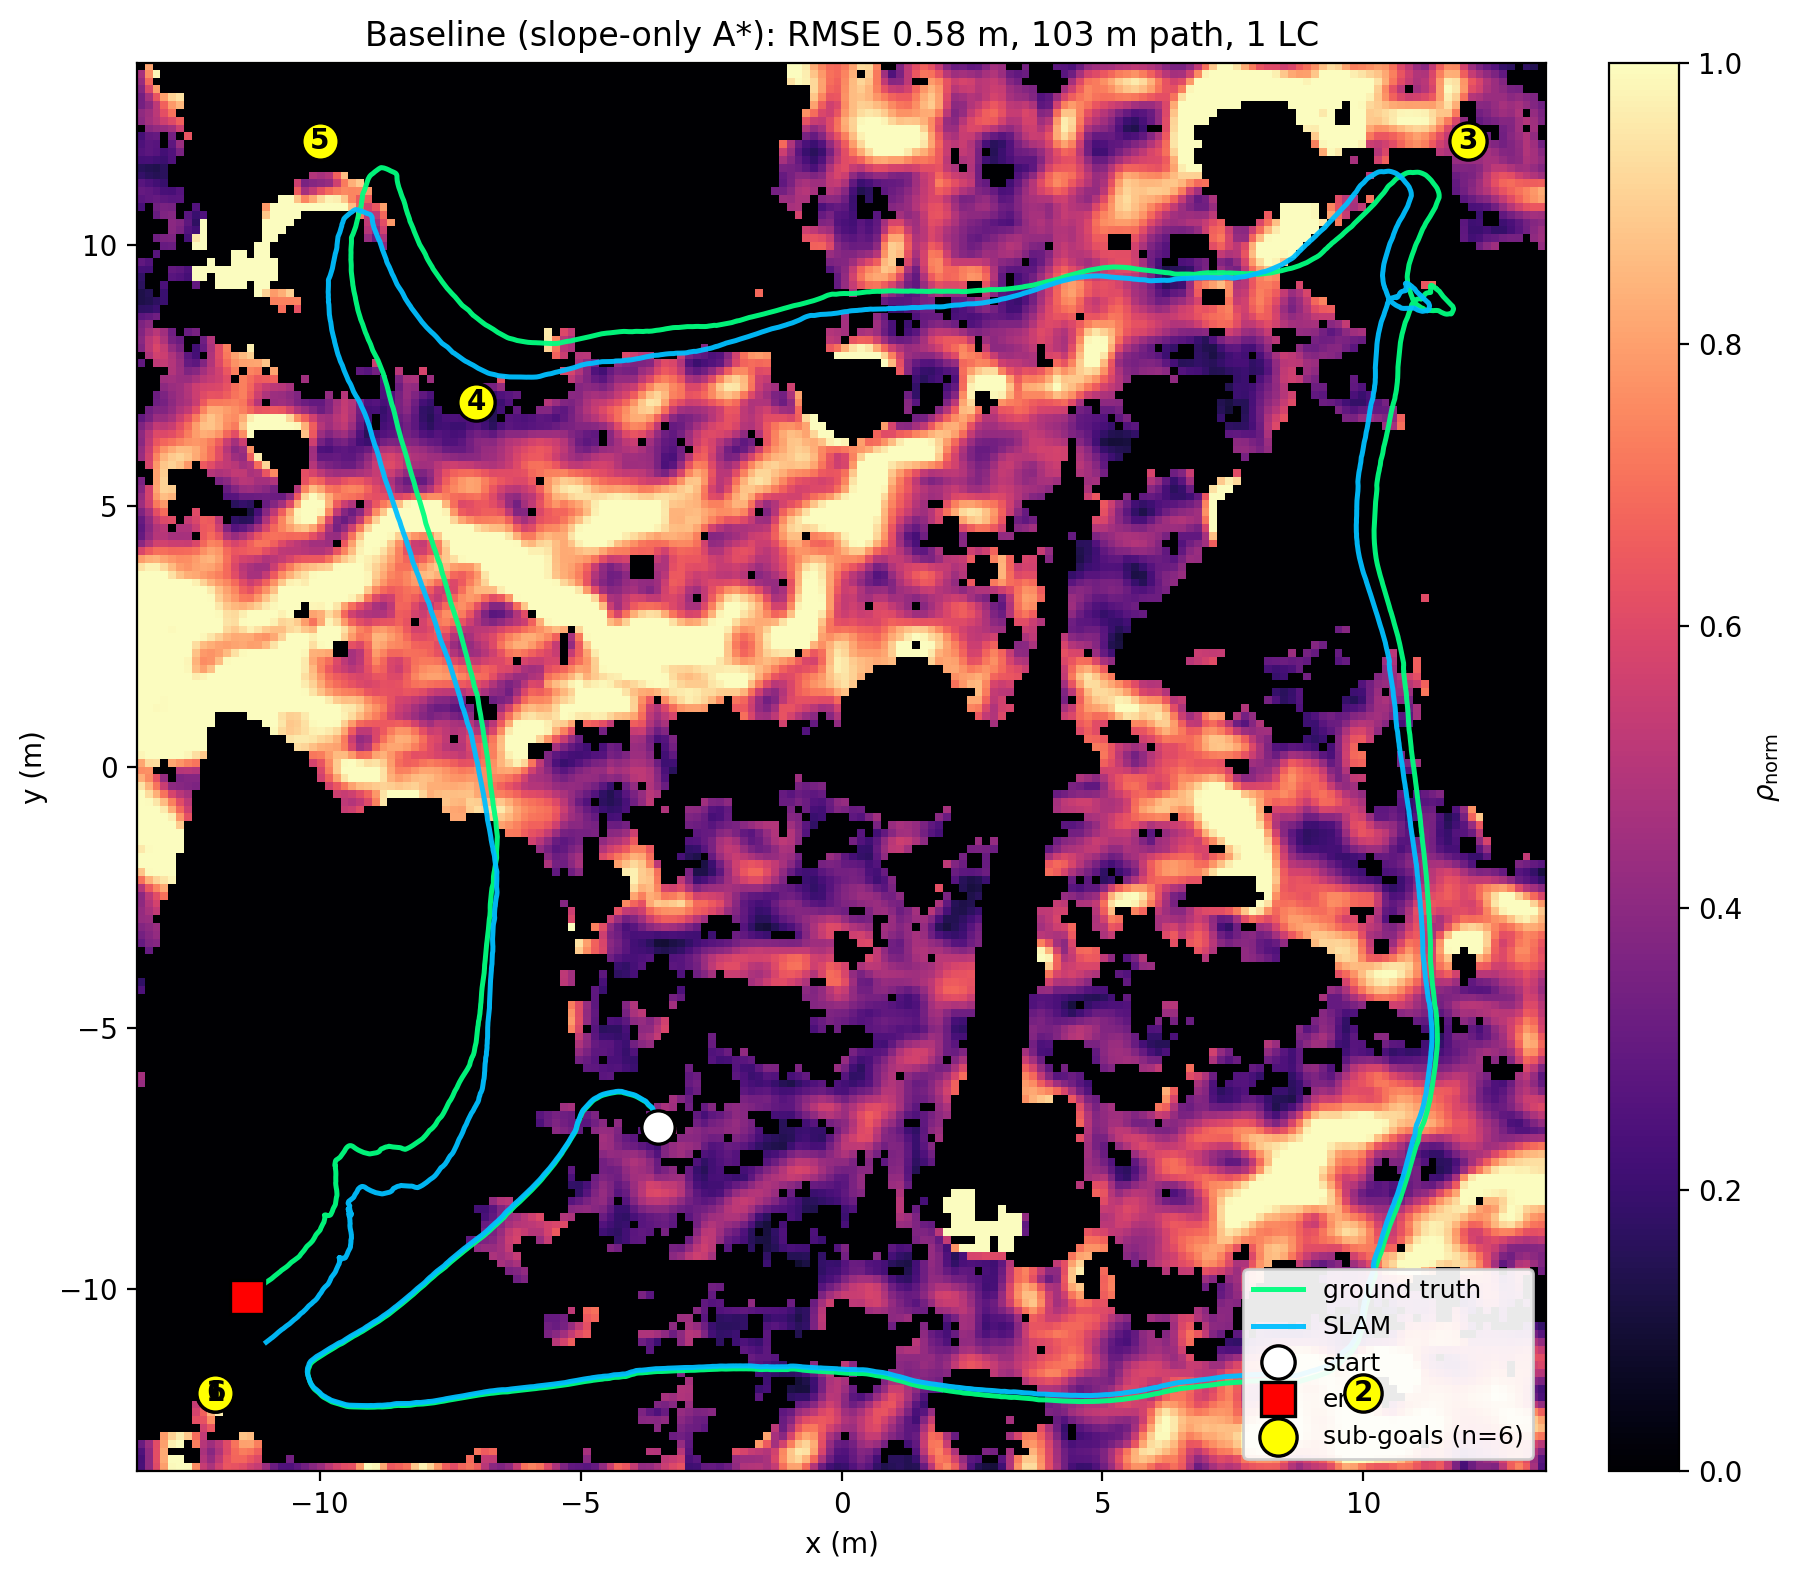
\includegraphics[width=\linewidth]{03_panel_baseline}
    \caption{Baseline (slope-only A*): RMSE 0.582~m, 0 detours, 1 LC.}
    \label{fig:traj_baseline}
\end{subfigure}\hfill
\begin{subfigure}[t]{0.48\linewidth}
    \centering
    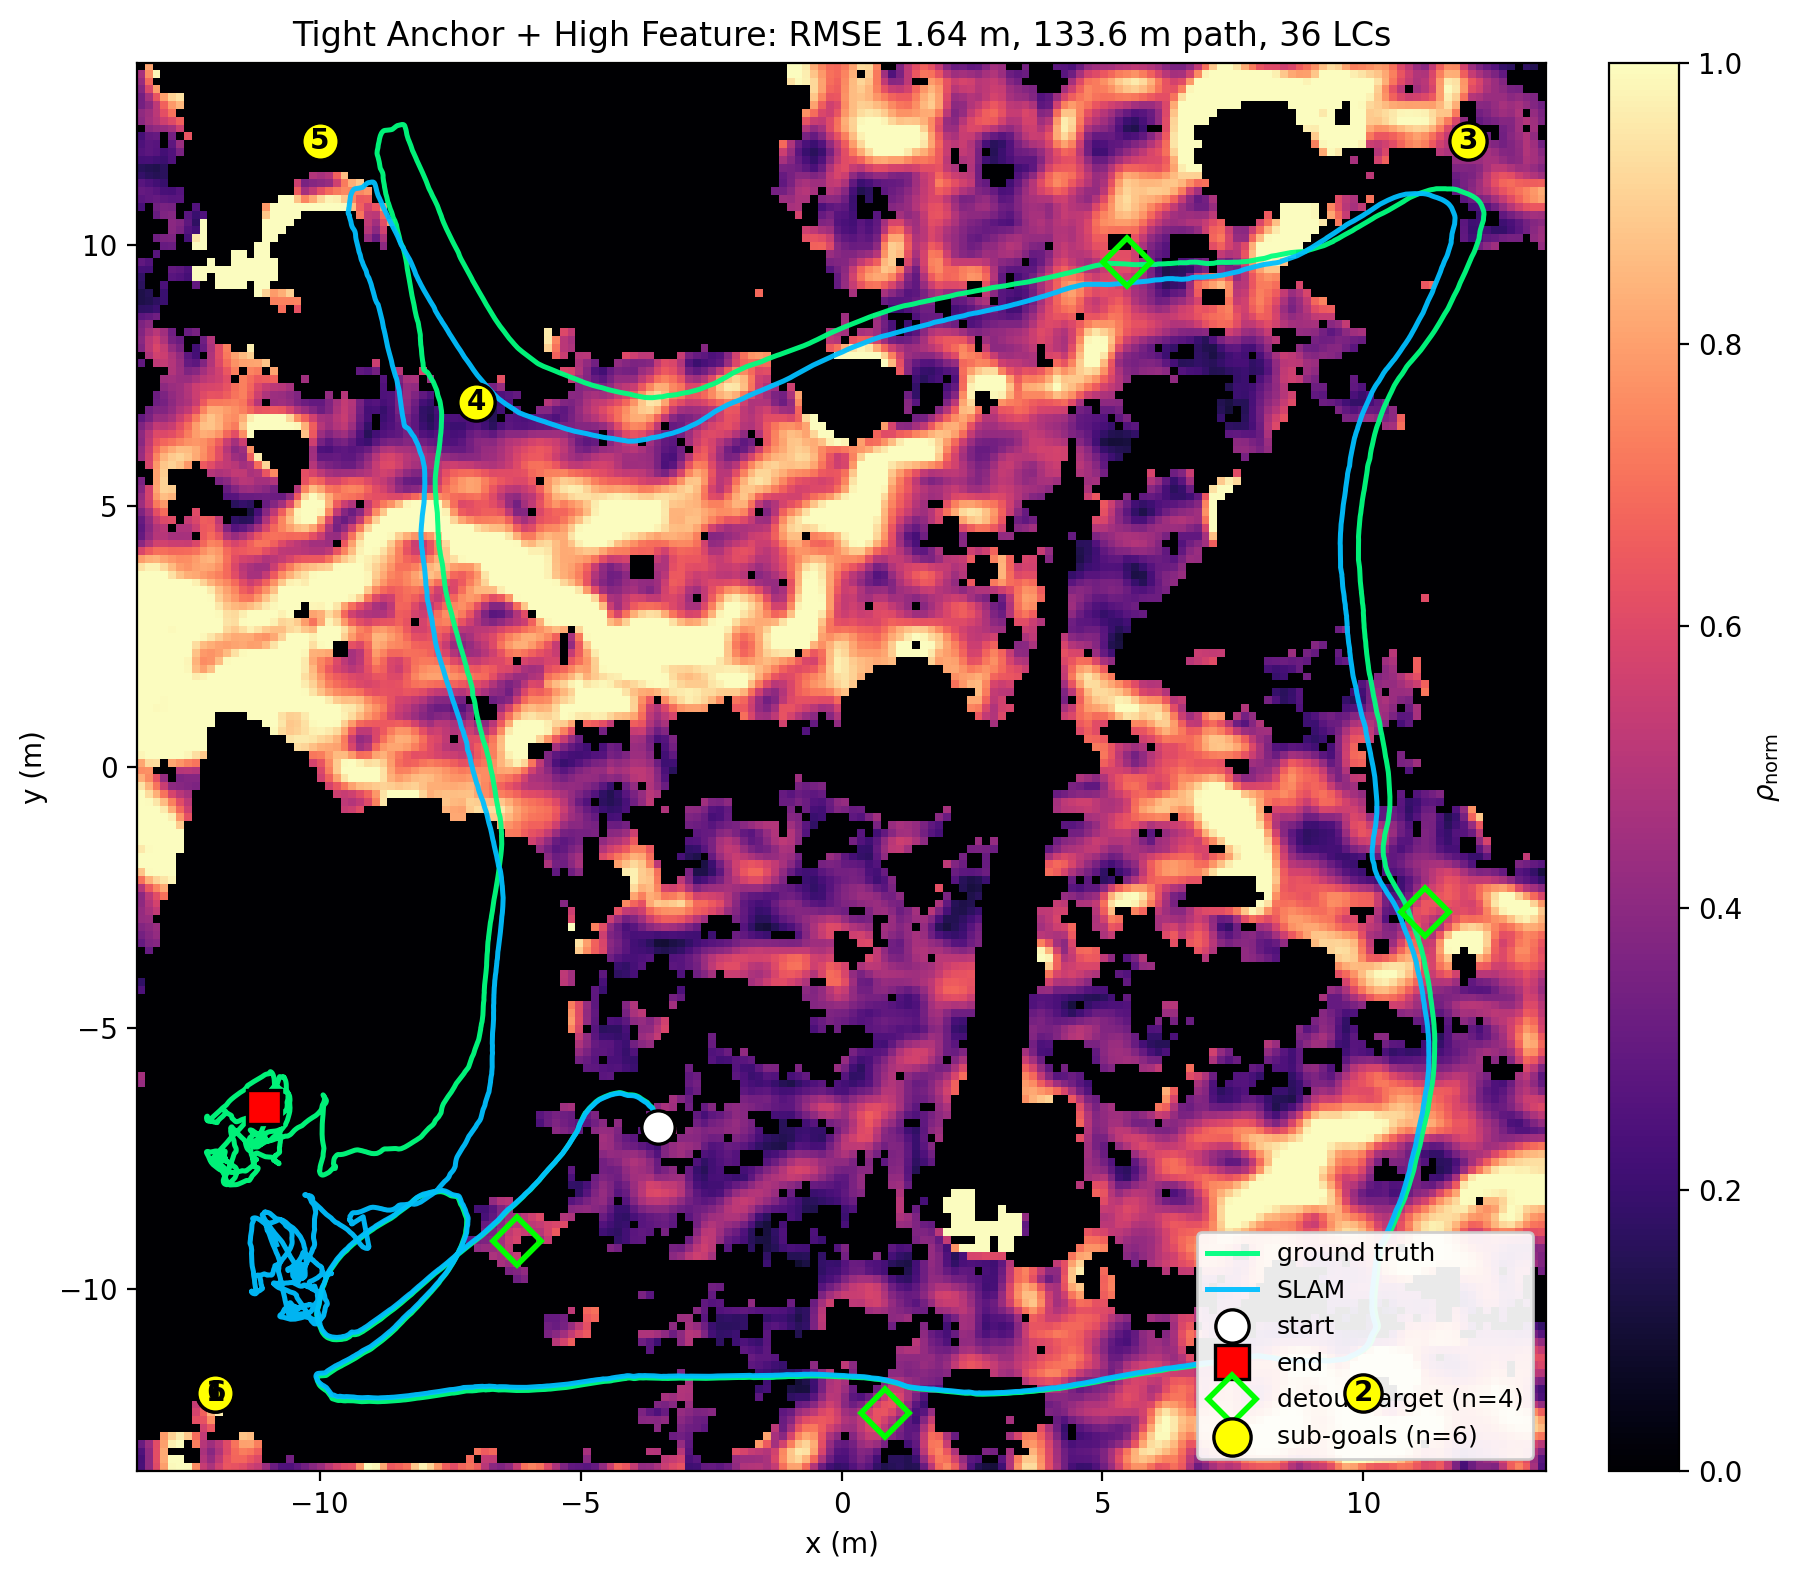
\includegraphics[width=\linewidth]{06_panel_tight_anchor_perc}
    \caption{Tight Anchor $+$ High Feature: RMSE 11.0~m; stalls on rocky anchor cells, 4/6 sub-goals.}
    \label{fig:traj_tight_anchor}
\end{subfigure}

\vspace{1mm}

\begin{subfigure}[t]{0.48\linewidth}
    \centering
    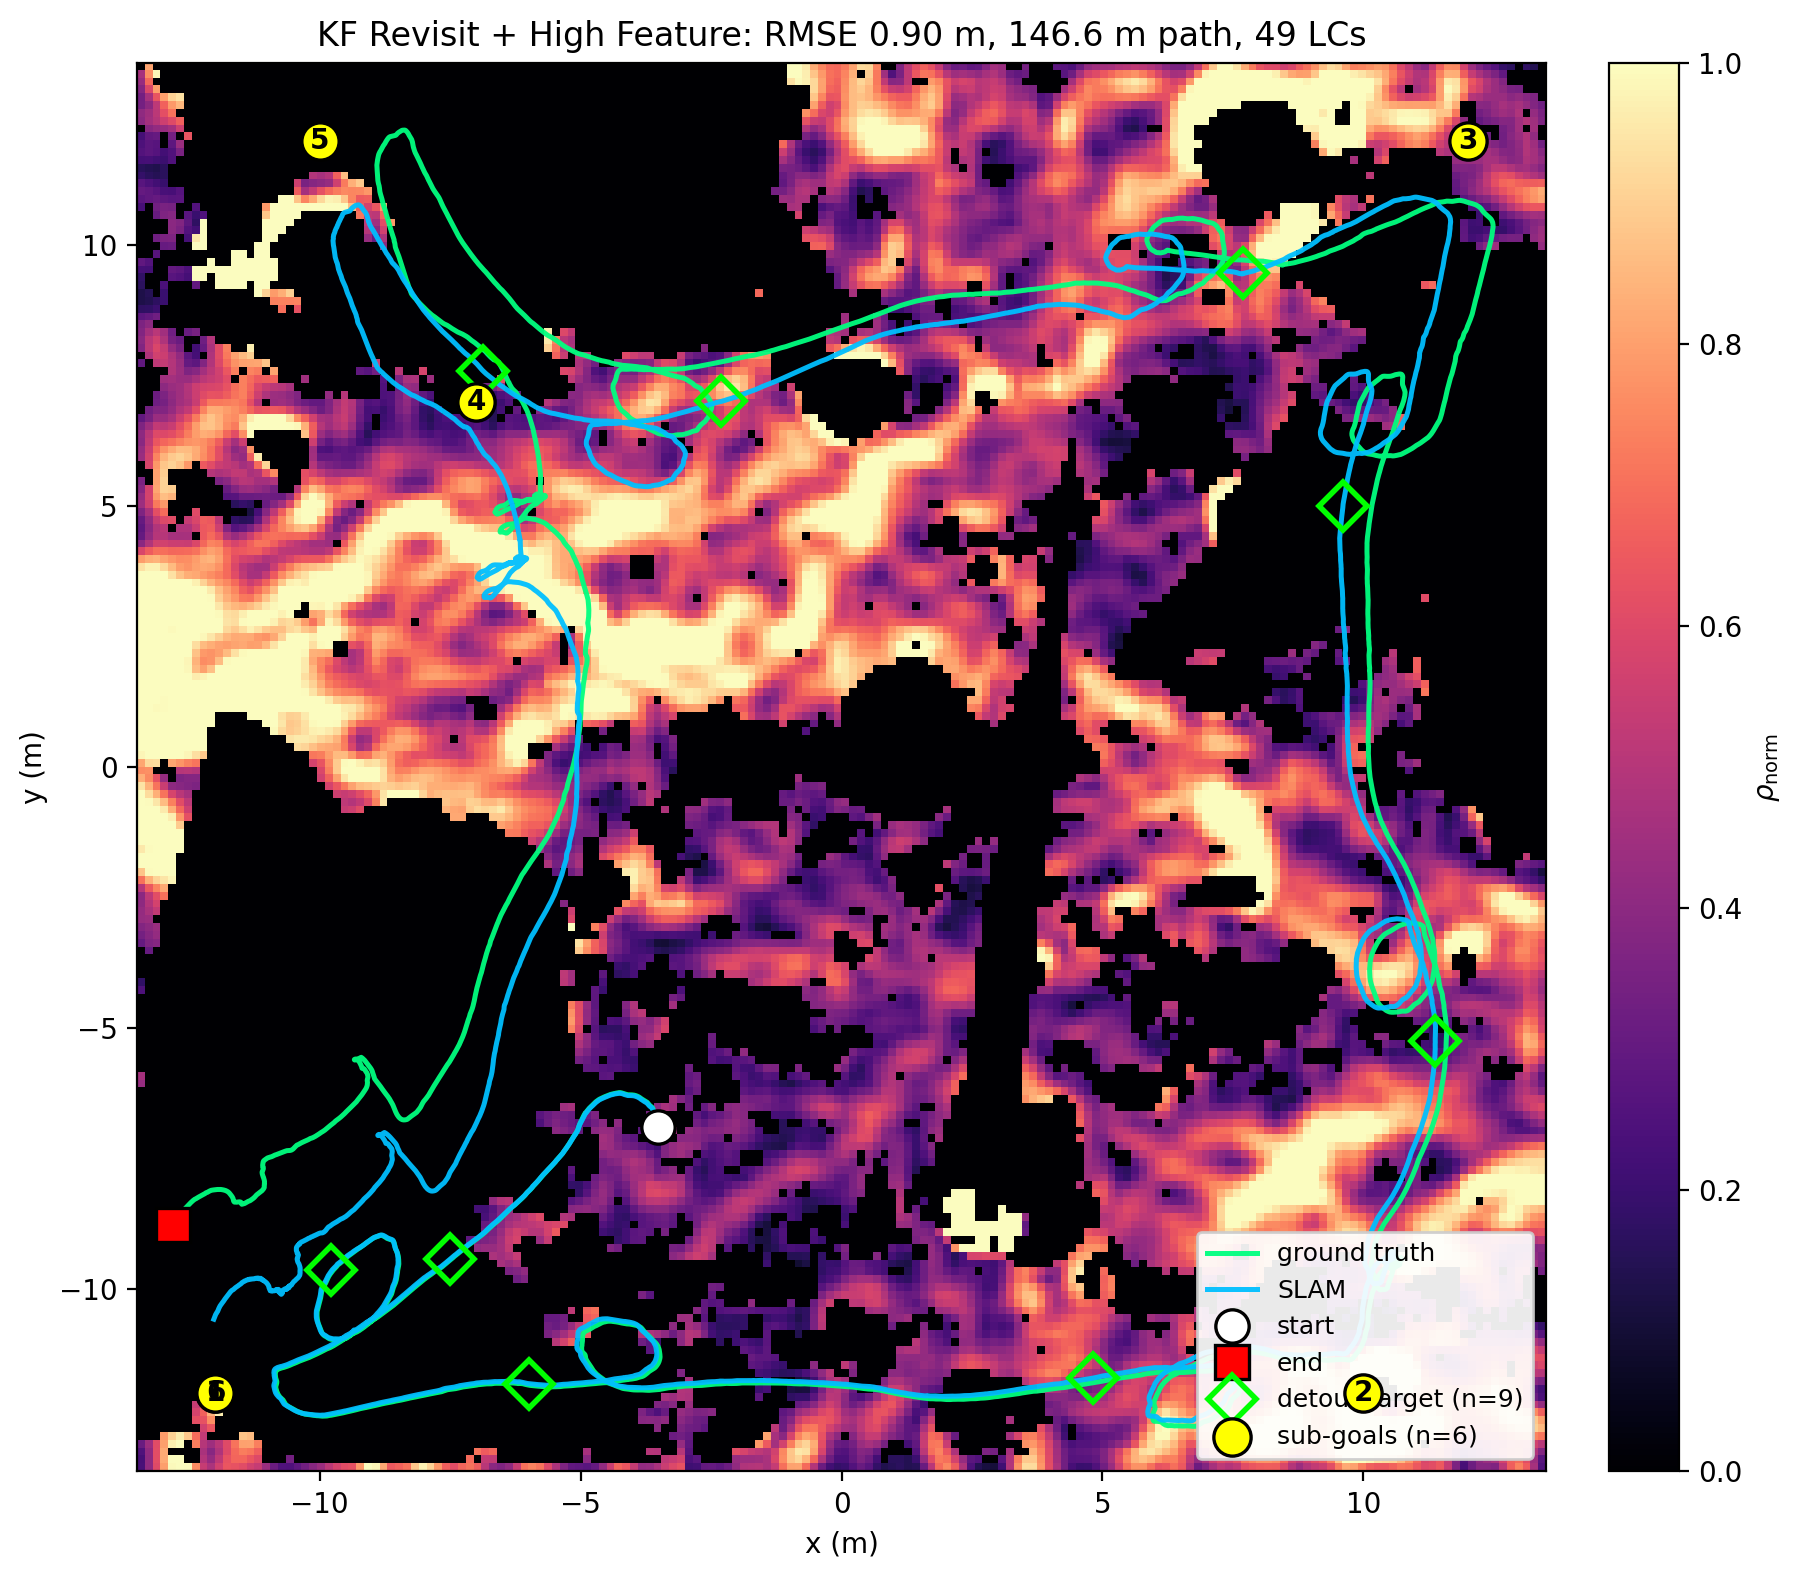
\includegraphics[width=\linewidth]{07_panel_kf_revisit_perc}
    \caption{KF Revisit $+$ High Feature: RMSE 0.905~m, 49 LCs, 9 detours; mobile but not yet winning.}
    \label{fig:traj_kf_perc}
\end{subfigure}\hfill
\begin{subfigure}[t]{0.48\linewidth}
    \centering
    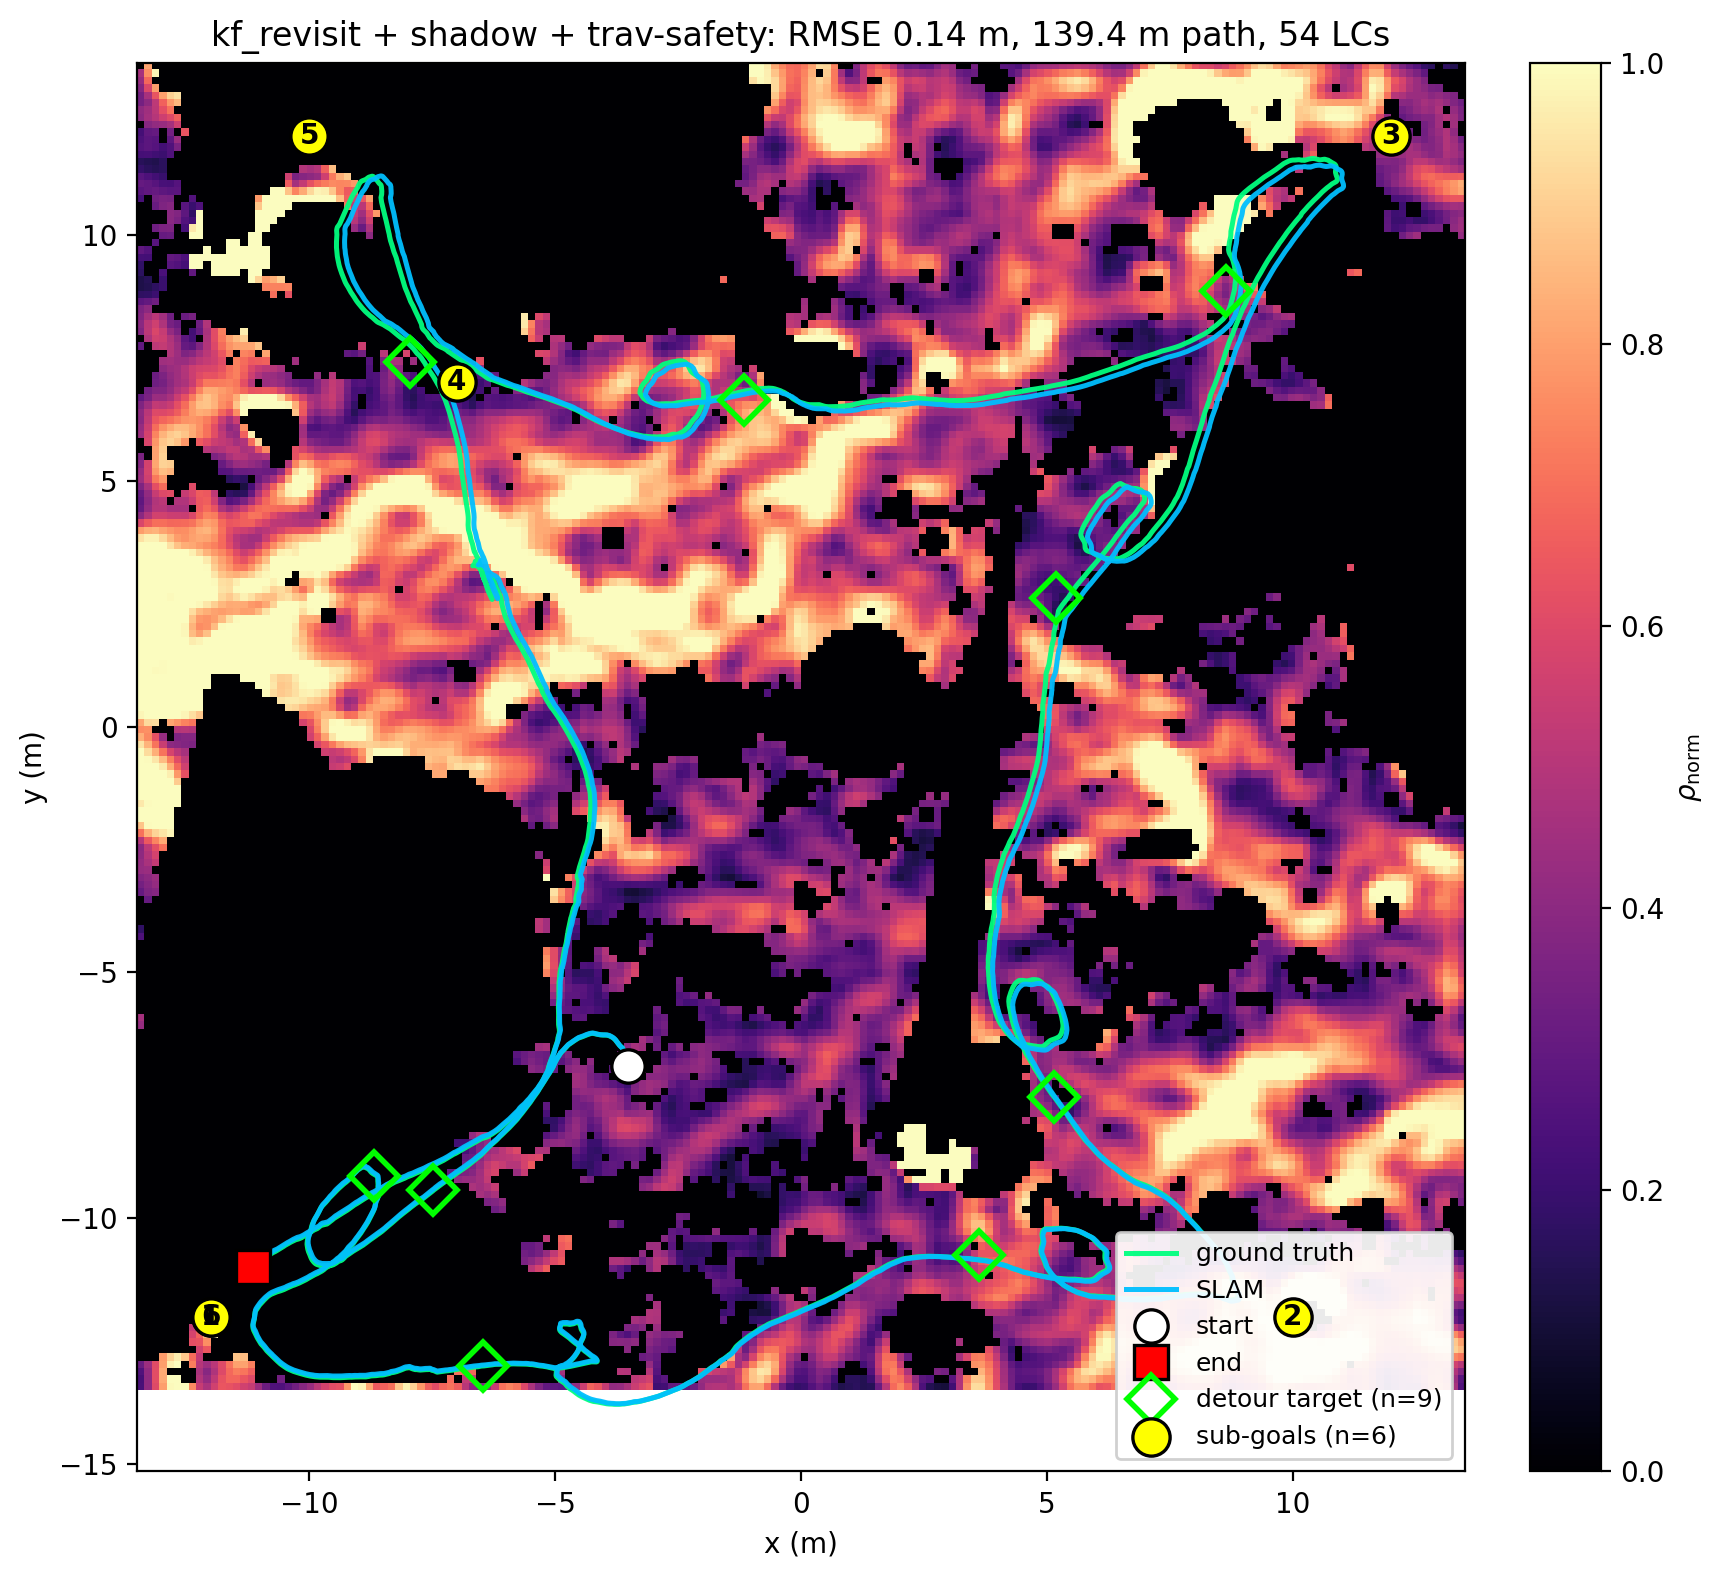
\includegraphics[width=\linewidth]{01_panel_winner}
    \caption{KF Rev.~$+$~Shadow~$+$~Safety (winner): RMSE 0.140~m, 54 LCs, 9 detours.}
    \label{fig:traj_winner}
\end{subfigure}

\caption{Ground-truth trajectories for four representative variants on the six-sub-goal tour (LAC preset~6), overlaid on the $\rho_{\text{norm}}$ field. Yellow numbered circles are sub-goals; green diamonds are detour targets (filled $=$ verified-success via a loop closure within 2~m). The winner (d) follows sunlit corridors and triggers KF revisits that produce a dense pattern of late-mission loop closures binding back to the first leg.}
\label{fig:trajectories}
\end{figure}

\subsection{Why This Combination Works: Mechanism Analysis}
\label{sec:mechanism}

The winner combines three mechanisms that each contribute distinct value, none of which is sufficient alone.

\textbf{(a) Shadow-aware cost keeps SLAM accurate.} With $s = 6$, the planned path routes through sunlit corridors. The winning trajectory spends only 15.3\% of its path-distance in shadow versus the baseline's 57.5\%. Shadowed cells produce no visual features, so reducing shadow exposure directly raises per-frame feature count and tightens VO. The downstream effect is structural: SLAM-estimated pose stays within \texttt{LC\_DIST\_THRESHOLD}~$=$~1~m of ground truth for longer, which means the geometric LC trigger \emph{keeps working} under realistic drift conditions rather than going blind once drift exceeds 1~m.

\textbf{(b) Traversability-as-safety prevents rocky-cell stalls.} With $w = 4$, the planner avoids cells where the local ArcPlanner would deadlock. Without this term, the Shadow-only variant (Table~\ref{tab:ablation}, row ``Shadow Avoidance / none'') reaches only four of six sub-goals and accumulates 3.07~m of RMSE; adding $w = 4$ produces the cleanest mobility profile of any tested variant (1\% stationary, zero stuck events).

\textbf{(c) KF Revisit detour actively engineers loop closures.} With $T_{\text{LC}} = 400$, the detour fires whenever SLAM has been drifting for roughly 400 keyframe updates without a loop closure. In the winning run, 9 detours fired and 54 loop closures resulted --- versus the baseline's single LC.

The structurally important finding: \textbf{20 of the 54 LCs in the winning variant bind back to keyframes in the first 10\% of the mission}, near the GTSAM prior pose at $X_0$; a further 28 fire in the last 20\% (during the return-to-start leg $g_5 \to g_6$). Cross-trajectory LCs that bind late keyframes to early keyframes --- which are themselves well-anchored to ground truth by the pose-graph prior initialization --- are what enables \emph{global} drift correction. Mid-trajectory LCs only constrain relative pose between temporally close keyframes and reduce only local drift. The combination of (a)~keeping SLAM accurate long enough to make the geometric LC trigger fire on the return leg, and (b)~actively driving the rover near old keyframes, is what produces the cross-trajectory bindings that anchor the late-mission pose graph back to the well-anchored start region.

\subsection{Full 3$\times$3 Ablation Matrix}

Table~\ref{tab:ablation} reports the complete 3$\times$3 ablation crossing the three global-cost configurations with three detour modes. Several cells fail outright. Three observations:

\begin{enumerate}
    \item \emph{The baseline global cost is fragile under aggressive detour mechanisms.} Pairing slope-only A* with Tight Anchor diverges catastrophically (RMSE 130.8~m); pairing it with KF Revisit reproduces a downstream LAC-stack sensor-dropout failure at step 894 (a $\texttt{KeyError}$ on the $\texttt{FrontLeft}$ camera input, not specific to our code).
    \item \emph{Tight Anchor is environment-sensitive.} It works with High Feature global cost (1.64~m RMSE, 36~LCs), times out under Shadow Avoidance, and diverges under the baseline. The cause is consistent: anchors are pre-computed from high-$\rho$ cells, which co-occur with rocky cells; without a heavy roughness penalty in the global cost ($w \ge 8$), the rover stalls trying to reach them.
    \item \emph{KF Revisit is the most robust detour mechanism.} It works with High Feature (0.90~m), with Shadow Avoidance (0.74~m), and produces the headline winner with Shadow~$+$~Safety (0.14~m). The reason is structural: KF Revisit targets keyframes the rover has \emph{already visited} --- driveable by construction --- rather than DEM-predicted cells.
\end{enumerate}

\begin{table}[t]
\renewcommand{\arraystretch}{1.25}
\caption{Full 3$\times$3 ablation matrix. Each cell reports SLAM RMSE / sub-goals reached / stationary~\%. Failed runs are flagged; the headline winner is in bold.}
\label{tab:ablation}
\centering
\small
\begin{tabular}{p{2.1cm}p{1.5cm}p{1.5cm}p{1.5cm}}
\toprule
Global cost & none & Tight Anchor & KF Revisit \\
\midrule
Baseline (slope only) & 0.58~/~6~/~1\% & 130.8~/~3~/~10\% \ding{55} & crashed \ding{55} \\
High Feature ($\beta{=}2,w{=}8$) & 1.59~/~6~/~10\% & 1.64~/~6~/~3\% & 0.90~/~6~/~3\% \\
Shadow Avoid. ($s{=}2$) & 3.07~/~4~/~1\% & timed out \ding{55} & 0.74~/~6~/~1\% \\
\textbf{Shadow $+$ Safety} ($s{=}6, w{=}4$) & --- & --- & \textbf{0.14~/~6~/~1\%} \\
\bottomrule
\end{tabular}
\end{table}

\subsection{Tight Anchor vs. KF Revisit: Collects vs. Causes}

A revealing detail: the \texttt{tight\_anchor\_perc} run fired 36 loop closures from only 4 detour attempts, while the \texttt{kf\_revisit\_perc} run fired 49 LCs from 9 detour attempts. Tight Anchor fires fewer detours in the first place because anchor candidates must pass three filters simultaneously (proximity to current pose, proximity to a past keyframe, not in the per-leg blacklist) and the pool of $K \le 12$ anchors often offers no valid candidate. The 36 LCs that \emph{did} fire in the Tight Anchor run were largely incidental --- the rover happened to pass within 1~m of a past keyframe during normal travel, not because the detour drove it there. By contrast, the winning KF Revisit run's 54 LCs came from 9 active detour attempts, with cross-trajectory bindings concentrated in the return leg. The intuition: \textbf{Tight Anchor collects loop closures; KF Revisit causes them.}

\subsection{Failure-Mode Analysis}

We report honest failure modes for the variants that did not complete.

\textbf{UE4 collision meshes invisible to the DEM.} The LAC simulator includes UE4 collision meshes (the lunar lander mesh at world origin; smaller crater meshes elsewhere) that are not represented in the DEM. The DEM-based cost cannot see them. A previous-tour Tight Anchor variant ended at $(+0.16, +7.55)$ having spent 1{,}877 consecutive frames in a 1.5~m radius --- a clear stuck cluster on a cell with sub-median roughness and zero rocks in the DEM rock grid. We removed the central $(0, 0)$ waypoint after determining that the lander mesh deadlocks the rover regardless of cost tuning.

\textbf{Simulator non-determinism near rocks.} The same baseline configuration produced RMSE 0.58~m on one run and 9.08~m on another, with identical waypoint output from the offline planner. The non-determinism is in the simulator's ArcPlanner-rock interaction; we report the best-completed baseline as the reference, noting this is the published number, not an average. A rigorous version of this experiment would average over $N \ge 5$ runs per variant.

\textbf{LAC sensor dropout.} The simulator occasionally fails to deliver a camera frame, and $\texttt{nav\_agent.run\_step()}$ indexes $\texttt{input\_data["Grayscale"][SensorPosition.FrontLeft]}$ without exception handling, terminating the mission with a $\texttt{KeyError}$. The \texttt{kf\_revisit\_base} variant crashed this way at step 894 --- an LAC-stack-level failure not specific to our code.

\subsection{Compute Footprint}

One tour run on preset~6 (RTX~3090, 24~GB VRAM, Xvfb headless rendering, 0.15--0.20$\times$ real-time sim ratio) takes 45--65~min for mobile variants. The full 10-variant matrix completes in 10--13~h of wall-clock time end-to-end. GPU memory is dominated by the UE4 simulator (~21~GB); the LightGlue and SuperPoint networks share the remainder. Earlier testing hit CUDA OOM on long missions until $\texttt{PYTORCH\_CUDA\_ALLOC\_CONF=expandable\_segments:True}$ was added to the launcher.


\section{Conclusion}
\label{sec:conclusion}

We demonstrated that path-planner-side loop-closure engineering is a viable mechanism for reducing SLAM drift on lunar-rover tour-style missions. On the LAC simulator, a composite \emph{Shadow~$+$~Safety} global cost combined with an online \emph{Keyframe-Revisit} detour achieves SLAM RMSE of 0.14~m on a 139.4~m tour --- a 4.16$\times$ absolute RMSE reduction and a 5.55$\times$ per-meter drift reduction over a slope-aware A* baseline, with no modifications to the SLAM backend.

Three mechanisms each contribute. First, a DEM-derived shadow-avoidance cost steers the planner through sunlit, feature-stable corridors, keeping the SLAM-estimated pose within the backend's 1~m geometric LC-trigger threshold long enough for loop closures to fire on the return leg. Second, a traversability-safety penalty avoids rocky cells where the local ArcPlanner deadlocks, eliminating residual stuck events. Third, the keyframe-revisit detour mechanism, triggered by elapsed-steps-since-last-LC, actively drives the rover near previously visited keyframes; 20 of the winning variant's 54 loop closures bind late-mission keyframes back to the first 10\% of the trajectory --- providing the cross-trajectory drift correction the heritage baseline cannot.

The structural lesson is that \emph{detour targets matter}. Keyframe-revisit targets are driveable by construction (the rover already went there) and LC-eligible by construction (the backend already stored a keyframe there), while DEM-predicted feature-rich anchors co-occur with the rocky cells the local controller cannot navigate. Tight Anchor \emph{collects} loop closures; KF Revisit \emph{causes} them.

\textbf{Limitations.} Three caveats. (i)~The published baseline RMSE is the best-completed run; we observed simulator non-determinism producing a 9.08~m result for the same configuration on a separate run, with identical offline-planner output. A rigorous version of this experiment should average over multiple runs per variant. (ii)~Results are reported on a single LAC preset (preset~6); the Phase~0 predictor was validated on preset~7. (iii)~DEM-driven planning is fundamentally blind to UE4 collision meshes not represented in the elevation model --- a limitation of the LAC simulator, but more broadly an argument for fusing DEM-based costs with runtime semantic segmentation in future work.


\section{Future Directions}
\label{sec:future}

In rough priority order:

\textbf{Smarter detour-target scoring.} The current scorer minimizes added detour distance. Three improvements suggest themselves: (a)~bias toward \emph{temporally old} keyframes near the GTSAM prior pose, to maximize the cross-trajectory drift-correction effect identified in Sec.~\ref{sec:mechanism}; (b)~score by stored feature count at the candidate keyframe (already available in $\texttt{backend.keyframe\_data}$), preferring targets with high LightGlue-match likelihood; (c)~score by $\rho_{\text{norm}}$ or shadow status at the candidate, preferring sunlit, feature-rich revisit cells.

\textbf{Appearance-based loop-closure search.} The dominant remaining structural limitation is that the LAC backend's loop-closure search is geometric: once SLAM drift exceeds 1~m, the trigger cannot detect a true revisit. An appearance-based search (DBoW3 with SuperPoint descriptors, or NetVLAD global descriptors) would expand the operational envelope of our detour mechanism. We deliberately avoided this for the present work to demonstrate that planner-side mechanisms alone suffice; it is the obvious next step.

\textbf{Validation on LRO-derived mid-scale terrain.} The DEM-derived predictor should be re-validated on real lunar terrain from the Lunar Reconnaissance Orbiter NAC co-registered with LOLA. A kilometer-scale traverse --- where the heritage planner's drift is dominant --- would strengthen the case for the approach beyond the synthetic LAC environment.

\textbf{Multi-run statistical evaluation.} Given the observed sim non-determinism, a publication-grade version of this work should report mean $\pm$ standard deviation over $N \ge 5$ runs per variant. The full five-variant matrix would take roughly 25 runs (10--15~h of compute) and is within an overnight schedule.

\textbf{Real-rover validation.} The approach taken here is directly portable to physical lunar-analog rovers operated by NASA JPL, ESA, and commercial teams on terrestrial test ranges: no SLAM-backend modifications are required, and the only a-priori inputs are a DEM and a sun direction.


\section*{acknowledgements}

The author thanks the Stanford NavLab for the LAC simulator and reference SLAM stack used in this work, and the AA278 course staff (Spring 2026) for guidance through the project lifecycle.


\section*{code availability}

All code, configurations, scripts, and result artifacts referenced in this paper are available at:
\begin{center}
\url{https://github.com/santiagothorup/Lunar_Perception_Aware_Planning}
\end{center}


\bibliographystyle{apalike}
\bibliography{my_bibliography_file}


\end{document}
